\title[Causality]{Causality: Lecture 12}
\author[Joris Mooij]{\\[5mm]\large Joris Mooij \& Patrick Forr\'e\\
\url{j.m.mooij@uva.nl}, \url{p.d.forre@uva.nl}}
\institute[UvA]{University of Amsterdam}
\date[2022-04-25]{\normalsize April 25th, 2022}
\maketitle

\begin{frame}{Twin SCM}
\begin{definition}
  We define the \emph{twinned SCM} $M^\twin = \ltuple \Sin \dot\cup \Sin', \Send \dot\cup \Send', \Srnd, \tilde{\CX}, P, \tilde{f} \rtuple$
  with 
  \begin{enumerate}
    \item $\Sin' = \{j' : j \in \Sin\}$ a copy of $\Sin$,
    \item $\Send' = \{v' : v \in \Send\}$ a copy of $\Send$, 
    \item the twinned domain given by
  $$\tilde{\CX} = \CXJ \times \CXJ \times \CXV \times \CXV \times \CXW$$
  (i.e., with $\CX_{\Sin'} = \CX_{\Sin}$ and $\CX_{\Send'} = \CX_{\Send}$),
    \item the twinned causal mechanism components given by
  $$\tilde{f}_v\big((x_J,x_{J'}),(x_V,x_{V'}),\xW\big) = 
  \begin{cases}
    f_v(\xJ,\xV,\xW) & v \in \Send,  \\
    f_v(x_{J'},x_{V'},\xW) & v \in \Send'.
  \end{cases}$$
  \end{enumerate}
\end{definition}
  This creates copies of some variables so that their values can differ in the counterfactual world with respect to the actual world.
\end{frame}

\begin{frame}{Properties of the twinning operation I}
The twinning operation has the following properties:
\begin{Prp}
Let $M = \lt \Sin, \Send, \Srnd, \CX, P, f \rt$ and $\tilde{M} = \ltuple \Sin, \Send, \Srnd, \CX, P, \tilde{f} \rtuple$ be SCMs.
  \begin{enumerate}
\item Twinning preserves equivalence: $M \equiv \tilde{M} \implies M^\twin \equiv \tilde{M}^\twin$.
\item 
For $L \subseteq V$ such that $M_{\doit(V\setminus L)}$ is uniquely solvable,
$$(M_{\setminus L})^\twin = (M^\twin)_{\setminus (L\cup L')}.$$
\item If $M$ is uniquely solvable, then $M^{\twin}$ is uniquely solvable.
\item If $M$ is simple, then $M^{\twin}$ is simple.
\end{enumerate}
\end{Prp}
%\begin{Lem}
%Let $M = \lt \Sin, \Send, \Srnd, \CX, P, f \rt$ be a simple SCM. Then
%$M$ and $M^\twin$ are interventionally equivalent w.r.t.\ $V \cup W$.
%\end{Lem}
\end{frame}

\begin{frame}{Properties of the twinning operation II}
Hard interventions are compatible with twinning:
\begin{Prp}
Let $M = \lt \Sin, \Send, \Srnd, \CX, P, f \rt$ be an SCM.
\begin{itemize}
  \item For $T \subseteq \Sin \cup \Send$ (sic!), $\xT \in \CXT$:
    $$(M^\twin)_{\doit(X_T=\xT,X_{T'}=\xT)} = (M_{\doit(\XT=\xT)})^\twin.$$
  \item For $T \subseteq \Srnd$ (sic!), $Q_T \in \prod_{t\in T} \C{P}(\CX_t)$:
    $$(M^\twin)_{\doit(X_T\sim Q_T)} = (M_{\doit(\XT\sim Q_T)})^\twin.$$
  \item For $T \subseteq \Sin \cup \Send$ (sic!):
    $$(M^\twin)_{\doit(T,T')} = (M_{\doit(T)})^\twin.$$
\end{itemize}
\end{Prp}
\end{frame}

\begin{frame}{Graphical twinning operation}
We can also define a twinning operation on graphs.
\begin{Def}\label{def:G_twinning}
  Let $G=\lt J,V \cup W,E\rt$ be a CDG such that $\Pa^G(W) = \emptyset$. Write $J' := \{j' : j \in J\}$
  and $V' := \{v' : v \in V\}$ for copies of $J$ and $V$.
  The \emph{twinned graph
  $G^{\twin(J,V)}$} is defined as the CDG $\ltuple J \dot\cup J', V \dot\cup V' \cup W, \tilde{E}\rtuple$ with directed edges
  \begin{equation*}\begin{split}
    \tilde{E} := E & \cup \{w \tuh v' : w \in W, v \in V, w \tuh v \in E\}\\
                   & \cup \{i' \tuh v' : i \in J \cup V, v \in V, i \tuh v \in E\}.
  \end{split}\end{equation*}
\end{Def}
In words, we copy the nodes $J \cup V$ (but not the nodes $W$) and copy the edges accordingly.
The graphical and the SCM twinning operations are compatible:
\begin{Prp}
  For SCM $M = \lt \Sin, \Send, \Srnd, \CX, P, f \rt$, $G(M)^{\twin(J\cup V)} = G(M^\twin).$
\end{Prp}
\end{frame}

\begin{frame}{Example}
  Consider SCM with exogenous input variable $X$, endogenous variable $Y$, exogenous random variable $W$, and
  structural equation:
  $$Y^{\doit(x)} = f(x,W)$$
  Twinning adds exogenous input variable $X'$, endogenous variable $Y'$, and structural equation
  $$(Y')^{\doit(x')} = f(x',W)$$

  \bigskip
  \begin{center}\begin{tikzpicture}
    \begin{scope}
      \node[varc] (X) at (0,0) {$X$};
      \node[var] (Y) at (0,-1.5) {$Y$};
      \node[varh] (W) at (1,-0.75) {$W$};
      \draw[arr] (X) to (Y);
      \draw[arrh] (W) to (Y);
      \node at (0.5,-2.3) {\small $G(M)$};
    \end{scope}
    \begin{scope}[xshift=5cm]
      \node[varc] (X) at (0,0) {$X$};
      \node[var] (Y) at (0,-1.5) {$Y$};
      \node[varh] (W) at (1,-0.75) {$W$};
      \draw[arr] (X) to (Y);
      \draw[arrh] (W) to (Y);
      \node[varc] (X2) at (2,0) {$X'$};
      \node[var] (Y2) at (2,-1.5) {$Y'$};
      \draw[arr] (X2) to (Y2);
      \draw[arrh] (W) to (Y2);
      \draw[dotted] (-1,-2) rectangle (1,0.5);
      \draw[dotted] (1,-2) rectangle (3,0.5);
      \node at (0,0.8) {\small factual};
      \node at (2,0.8) {\small counterfactual};
      \node at (1,-2.3) {\small $G(M^{\twin}) = G(M)^{\twin(X,Y)}$};
    \end{scope}
  \end{tikzpicture}\end{center}
\end{frame}

\part{Counterfactual Equivalence}
\frame{\partpage}

\begin{frame}{Counterfactual equivalence: definition}
\begin{definition}
  Let $M = \lt \Sin, \Send, \Srnd, \CX, P, f \rt$ and
  $\tilde{M} = \ltuple \tilde{\Sin}, \tilde{\Send}, \tilde{\Srnd}, \tilde{\CX}, \tilde{P}, \tilde{f} \rtuple$ be two simple SCMs
  and $O \subseteq (\Send \cap \tilde{\Send}) \cup (\Srnd \cap \tilde{\Srnd})$ a subset.
  We say that:
  \begin{enumerate}
    \item {\color{gray}$M$ and $\tilde{M}$ are \emph{observationally equivalent w.r.t.\ $O$} if $\CX_O = \tilde{\CX}_O$, $J = \tilde{J}$, $\CX_J = \tilde{\CX}_J$ and $P_{M}(X_O \mid \doit(\XJ)) = P_{\tilde{M}}(X_O \mid \doit(\XJ))$;}
    \item {\color{gray}$M$ and $\tilde{M}$ are \emph{interventionally equivalent w.r.t.\ $O$} if for every subset $T \subseteq O$ the intervened SCMs $M_{\doit(T)}$ and $\tilde{M}_{\doit(T)}$ are observationally equivalent w.r.t.\ $O \setminus T$;}
    \item $M$ and $\tilde{M}$ are said to be \emph{counterfactually equivalent w.r.t.\ $O$} if the twin SCMs $M^\twin$ and $\tilde{M}^\twin$ are interventionally equivalent w.r.t.\ $O \cup O'$, where
  $O'$ is the copy of $O$ in $\Send' \cap \tilde{\Send}'$.
  \end{enumerate}
%  In case the variables in $(V \cup W) \setminus O$ are considered latent, we sometimes omit the ``w.r.t.\ $O$'' in this terminology (i.e., we call $M$ and $\tilde{M}$ observationally equivalent, interventionally equivalent and counterfactually equivalent, respectively).
\end{definition}
\end{frame}

\begin{frame}{Marginalization preserves counterfactual semantics}
\begin{Thm}
  If $M$ is simple, $L \subseteq \Send$, and
  $M_{\setminus L}$ is its marginalization over $L$. Then $M$ and $M_{\setminus L}$ are {\color{gray}observationally,
  interventionally} and counterfactually equivalent w.r.t.\ $(V \cup W) \setminus L$.
\end{Thm}
\begin{proof}
  Write $K := V \setminus L$.
  Note that $(M_{\setminus L})^\twin = (M^\twin)_{\setminus (L \cup L')}$. 
  Since $M^\twin$ and its marginalization
  $(M^\twin)_{\setminus (L \cup L')}$ are interventionally equivalent w.r.t.\ $K \cup K' \cup W$,
  $M$ and $M_{\setminus L}$ are counterfactually equivalent w.r.t.\ $K \cup W$.
\end{proof}
Note: this can be shown for general (non-simple) SCMs as well.
\end{frame}

\begin{frame}{Implications between equivalences}
\begin{block}{Proposition}
  For simple SCMs $M, \tilde{M}$ and a subset $O \subseteq (\Send \cap \tilde{\Send}) \cup (\Srnd \cap \tilde{\Srnd})$:
  \begin{enumerate}
    \item If $M \equiv \tilde{M}$ then $M$ and $\tilde{M}$ are counterfactually equivalent w.r.t.\ $O$;
    \item If $M$ and $\tilde{M}$ are counterfactually equivalent w.r.t.\ $O$ then 
      $M$ and $\tilde{M}$ are interventionally equivalent w.r.t.\ $O$;
    \item {\color{gray}If $M$ and $\tilde{M}$ are interventionally equivalent w.r.t.\ $O$ then 
      $M$ and $\tilde{M}$ are observationally equivalent w.r.t.\ $O$.}
  \end{enumerate}
\end{block}
The reverse implications do not hold in general. This expresses that causal modeling is more refined than
probabilistic modeling, and counterfactual modeling is more refined than interventional modeling.
\end{frame}

\begin{frame}{Pearl's Ladder of Causation}
  \centering
  \begin{tikzpicture}
    \node (0,0) {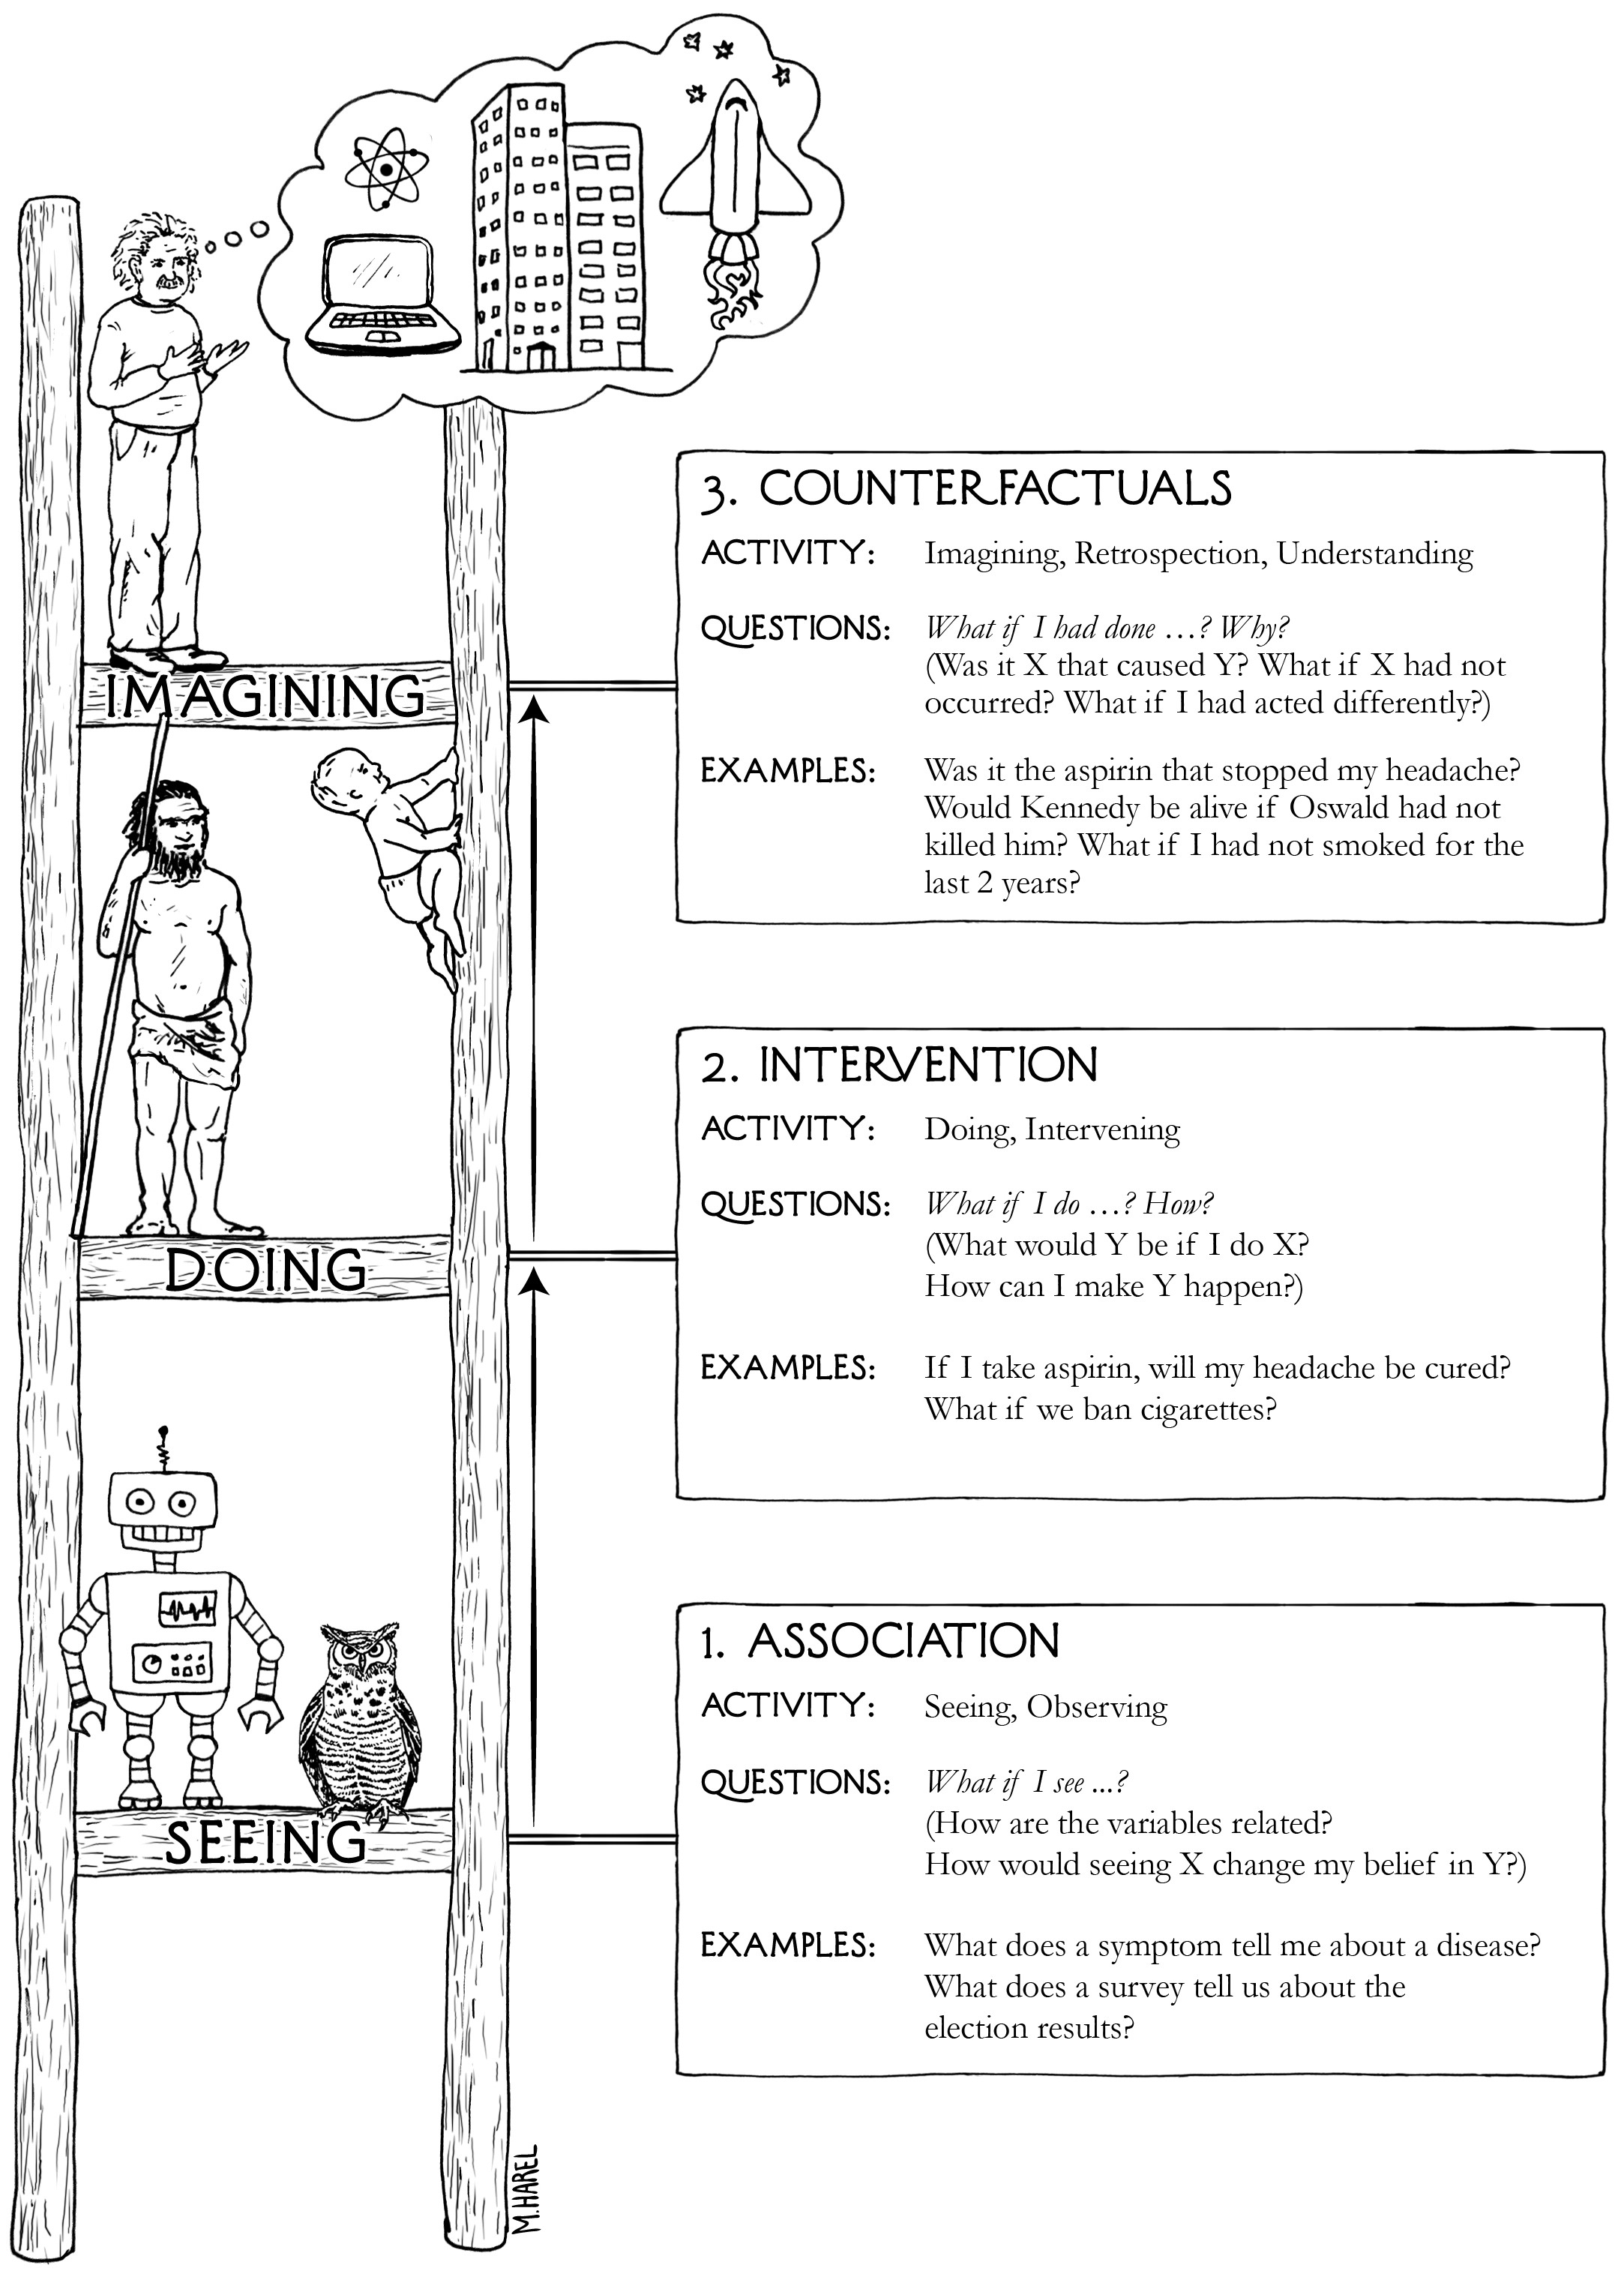
\includegraphics[width=0.45\textwidth]{ladder.jpg}};
    \draw[line width=1mm,fill=green,draw=green,->] (-4,2) -- node[below,sloped] {data-driven} (-4,-2);
    \draw[line width=1mm,fill=red,draw=red,->] (4,-2) -- node[below,sloped] {model-based} (4,2);
  \end{tikzpicture}
  \centerline{\tiny Image from Pearl \& Mackenzie, {\it The Book of Why}}
\end{frame}

\begin{frame}{Counterexample (Dawid, 2002)}
\begin{example}[1/2]
  For parameter $\rho\in[0,1]$, consider the SCM $M_\rho$ with binary exogenous input variable $X \in \{0,1\}$, endogenous variable $Y \in \RN$, a single latent exogenous random variable $W = (W_1,W_2) \in \RN^2$ with
exogenous distribution 
  $$\begin{pmatrix} W_1 \\ W_2 \end{pmatrix}\sim\C{N}\left(\begin{pmatrix}0 \\ 0\end{pmatrix},\begin{pmatrix}1&\rho\\ \rho&1\end{pmatrix}\right)$$
and structural equation
  $$Y^{\doit(x)} = W_1 (1 - x) + W_2 x.$$
  In a medical setting, this SCM could be used to model whether a patient was treated or not ($x=1$ vs.\ $x=0$) and the corresponding outcome for that patient ($Y^{\doit(x=1)}$ vs.\ $Y^{\doit(x=0)}$).
  Its interventional Markov kernel (that could be estimated with a randomized controlled trial) is given by
  $$P(Y = y \given \doit(X=x)) = \C{N}(y \given 0,1).$$
\end{example}
\end{frame}

\begin{frame}{Counterexample (Dawid, 2002)}
\begin{example}[2/2]
  Suppose in the factual world, $x = 0$ and $Y^{\doit(x=0)} = y \in \RN$.
  Consider the counterfactual: {\it ``What would the outcome have been, had we assigned treatment to this patient?''}.

  Construct the twin SCM $M_{\rho}^{\twin}$.
  The counterfactual query then asks for $P((Y')^{\doit(x'=1)}=y'\mid Y^{\doit(x=0)}=y)$. One can calculate that
$$
  P\big((Y')^{\doit(x'=1)},Y^{\doit(x=0)}\big) = \C{N}\left(\begin{pmatrix}0\\ 0\end{pmatrix}, \begin{pmatrix} 1 & \rho \\ \rho & 1 \end{pmatrix}\right)
$$
  and hence $P((Y')^{\doit(x'=1)} \mid Y^{\doit(x=0)}=y) = \C{N}(\rho y,1-\rho^2)$. 
  However: $\rho$ \alert{cannot be identified} from the Markov kernel $P(Y\given \doit X)$, since this is independent of $\rho$. 
  SCMs $M_{\rho}$ and $M_{\rho'}$ with $\rho\neq\rho'$ are interventionally equivalent, but not counterfactually equivalent.
%If we obtain the SCM from a reduction, we find the one with $\rho = 1$.
\end{example}
Take-home message: counterfactuals may be unidentifiable from data alone!
\end{frame}

\begin{frame}{Bounding counterfactuals (Balke \& Pearl, 1994)}
\begin{example}[1/2]
  For parameter $\rho\in\Delta_3=\{r=(r_{00},r_{01},r_{10},r_{11}) \in [0,1]^4 : r_{00}+r_{01}+r_{10}+r_{11}= 1\}$, consider the SCM $M_\rho$ with binary exogenous input variable $X \in \{0,1\}$, binary endogenous variable $Y \in \{0,1\}$, a single latent exogenous random variable $W \in \C{X}_W := \{00,01,10,11\}$ with exogenous distribution $P(W=w) = \rho_w$,
and structural equation
  $$Y^{\doit(x)} = f_{W}(x),$$
where we defined functions $f_{00},f_{01},f_{10},f_{11} : \{0,1\} \to \{0,1\}$ by:
  \begin{center}\begin{tabular}{c|llll}
    $x$ & $f_{00}(x)$ & $f_{01}(x)$ & $f_{10}(x)$ & $f_{11}(x)$ \\
    \hline
    0   & 0           & 0           & 1           & 1 \\
    1   & 0           & 1           & 0           & 1 
  \end{tabular}\end{center}

  Consider the counterfactual probability $P((Y')^{\doit(x'=1)}=1\mid Y^{\doit(x=0)}=0)$. 
\end{example}
\end{frame}

\begin{frame}{Bounding counterfactuals (Balke \& Pearl, 1994)}
\begin{example}[2/2]
%  We can update the distribution of $W$ with the observed outcome:
%  $$P_{M_{\rho}^{\twin}}(W | Y^{\doit(x=0)}=0) = (\rho_{00} / (\rho_{00} + \rho_{01}),\rho_{01} / (\rho_{00} + \rho_{01}),0,0).$$
%  $$P((Y')^{\doit(1)} = 1 | Y^{\doit(0)}=0) = \rho_{01} / (\rho_{00} + \rho_{01}).$$
Introduce the shorthand $p_{y|x} := P(Y=y\given \doit(X=x))$. This Markov kernel is given explicitly by:
  \begin{center}\begin{tabular}{ccl}
    $x$ & $y$ & $p_{y|x}$ \\
    \hline
    0   & 0   & $\rho_{00} + \rho_{01}$ \\ % = 1-eps
    0   & 1   & $\rho_{10} + \rho_{11}$ \\ %= eps
    1   & 0   & $\rho_{00} + \rho_{10}$ \\ %= delta
    1   & 1   & $\rho_{01} + \rho_{11}$ \\ %= 1-delta
  \end{tabular}\end{center}
We can derive the following bound:
%$$p_{0|0} - \min(p_{0|0},p_{0|1}) \le \rho_{01} \le \min(p_{0|0},p_{1|1})$$
%Hence
$$\small \frac{p_{0|0} - \min(p_{0|0},p_{0|1})}{p_{0|0}} \le P((Y')^{\doit(x=1)} = 1 | Y^{\doit(x=0)}=0) \le \frac{\min(p_{0|0},p_{1|1})}{p_{0|0}}$$
\end{example}

Example: almost-deterministic case ($p_{0|0} \approx 1$ and $p_{1|1} \approx 1$).
%Then $\rho_{01} \approx 0$, while $\rho_{00} + \rho_{01} \approx 1$.
Then the bound tells us that $P((Y')^{\doit(x=1)} = 1 | Y^{\doit(x=0)}=0) \approx 1$.
\end{frame}

\part{Causal Discovery: The Basics}
\frame{\partpage}

\begin{frame}{Outline}
  We give mathematical definitions for:
  \begin{itemize}
    \item $a$ causes $b$;
    \item $a$ is a direct cause of $b$;
    \item $a$ and $b$ have a common cause
  \end{itemize}
  and relate this to properties of the observational/interventional Markov kernels.

  \medskip
  We then study three causal discovery methods:
  \begin{enumerate}
    \item Randomized Controlled Trials
    \item Local Causal Discovery
    \item Y-structures
  \end{enumerate}

  \bigskip
  In the following slides, we always assume that
  $M = \lt \Sin, \Send, \Srnd, \CX, P, f \rt$ is a simple SCM with graph $G = G(M)$.

  \bigskip
  For IL-CBNs, everything can be done analogously.
\end{frame}

\begin{frame}{Defining Causal Relations}\label{frame:causes}
\begin{Def}
  If $a \in \Anc^G(b)\sm \{b\}$ for $a, b \in J \cup V \cup W$ we say that \emph{$a$ is a cause of $b$ according to $M$}.
\end{Def}
Only if $a$ causes $b$ according to $M$, a hard intervention on $a$ can change the distribution of $b$: 
\begin{Prp}
  Let $a \in V \cup W \cup J$ and $b \in V$.
  If $a \notin \Anc^G(b)$, then:
  $$P_{M}(X_b \given \doit(X_{J\sm \{a\}}),\doit(X_a)) = P_{M}(X_b \given \doit(X_{J\setminus \{a\}})).$$
\end{Prp}
\begin{proof}
  Application of rule 3 of the do-calculus.
\end{proof}
\end{frame}

\begin{frame}{Detecting Causal Relations}
This leads to a practical way of detecting the presence of a causal relation.
\begin{Cor}
  Let $b \in V$.
  For $a \in V \cup W \cup J$ with $a \ne b$, if
  there exist $x_{J\sm\{a\}} \in \CX_{J\sm\{a\}}$, $x_a,x_a' \in \CX_a$ s.t.\
      \begin{equation*}\begin{split}
        & P_{M}(X_b \given \doit(X_a=x_a),\doit(X_{J\setminus \{a\}}=x_{J\setminus \{a\}})) \\
        {} \ne {} & P_{M}(X_b \given \doit(X_a=x_a'),\doit(X_{J\setminus\{a\}}=x_{J\setminus\{a\}})),
      \end{split}\end{equation*}
  then $a$ is a cause of $b$ according to $M$, that is, $a \in \Anc^{G(M)}(b)$.

  Also, for $a \in V \cup W$ with $a \ne b$, if
  there exist $x_J \in \CX_J$, $x_a \in \CX_a$ s.t.\
  $$P_{M}(X_b \given \doit(X_a=x_a),\doit(X_J=x_J)) \ne P_{M}(X_b \given \doit(X_J=x_J)),$$
  then $a$ is a cause of $b$ according to $M$.  
\end{Cor}
This condition is sufficient, but not necessary.
\end{frame}

\begin{frame}{Defining Direct Causal Relations}
The notion of direct causation is always relative to some set of variables.
\begin{Def}
  If $a \in \Pa^G(b)$ for $a, b \in J \cup V \cup W$ with $a\ne b$ we say that \emph{$a$ is a direct cause of $b$ w.r.t.\ $V \cup W \cup J$ according to $M$}.
\end{Def}
This property is not necessarily preserved under marginalization!

\bigskip
Direct causation can be expressed in terms of causation in an intervened SCM:
\begin{Prp}
  For $a,b \in J \cup V \cup W$, $a$ is a direct cause of $b$ w.r.t.\ $J \cup V \cup W$ according to $M$ if and only if $a$ is a cause of $b$ according to $M_{\doit(V\setminus\{a,b\})}$.
\end{Prp}
\end{frame}

\begin{frame}{Detecting Direct Causal Relations}
The following is sufficient, but not necessary.
\begin{Cor}
  Let $b \in V$.
  For $a \in V \cup W \cup J$ with $a \ne b$, if there exist values $x_{J\setminus\{a\}} \in \CX_{J\sm\{a\}}$, $x_{V\setminus\{a,b\}} \in \CX_{V\setminus\{a,b\}}$, $x_a,x_a' \in \CX_a$ s.t.\
      \begin{equation*}\begin{split}
        & P_{M}(X_b \given \doit(X_a=x_a),\doit(X_{V\setminus\{a,b\}}=x_{V\setminus\{a,b\}}),\doit(X_{J\setminus \{a\}}=x_{J\setminus \{a\}})) \\
        {} \ne {} & P_{M}(X_b \given \doit(X_a=x_a'),\doit(X_{V\setminus\{a,b\}}=x_{V\setminus\{a,b\}}),\doit(X_{J\setminus\{a\}}=x_{J\setminus\{a\}})),
      \end{split}\end{equation*}
  then $a$ is a direct cause of $b$ w.r.t.\ $V \cup J \cup W$ according to $M$, i.e., $a \in \Pa^{G(M)}(b)$.

  Also, for $a \in V \cup W$ with $a \ne b$, if there exist values $x_J \in \CX_J$, $x_{V\setminus\{a,b\}} \in \CX_{V\setminus\{a,b\}}$, $x_a \in \CX_a$ such that
      \begin{equation*}\begin{split}
        & P_{M}(X_b \given \doit(X_a=x_a),\doit(X_{V\setminus\{a,b\}}=x_{V\setminus\{a,b\}}),\doit(X_J=x_J)) \\
        {} \ne {} & P_{M}(X_b \given \doit(X_{V\setminus\{a,b\}}=x_{V\setminus\{a,b\}}),\doit(X_J=x_J)),
      \end{split}\end{equation*}
  then $a$ is a direct cause of $b$ w.r.t.\ $V \cup J \cup W$ according to $M$.
\end{Cor}
\end{frame}

\begin{frame}{Forks}
  \begin{Def}
    Let $G = \lt J, V, E, L \rt$ be a CDMG. 
    A \emph{fork} from $v$ to $w$ in $G$ is a walk of the form:
        \[v=v_0 \hut v_1 \hut  \cdots \hut v_{k-1} \hus v_k  \tuh \cdots \tuh v_{n-1} \tuh v_n=w,\]
   %             \[v=v_0 \hut v_1 \hut  \cdots \hut v_{k-1} \huh v_k  \tuh \cdots \tuh v_{n-1} \tuh v_n=w,\]
        such that $v \ne w$, the walk contains both endnodes exactly once, 
        every node has at most one arrow head pointing towards it, and 
        both endnodes have an arrow head pointing towards them. 
    If the edge $v_{k-1} \hus v_k$ is directed ($v_{k-1} \hut v_k$) then we say that the fork has \emph{source} $v_{k}$.
  \end{Def}
\begin{Prp}
  Let $G = \lt J, V, E \rt$ be a CDG. For $a, b \in V$:
  there exists a fork between $a$ and $b$ in $G$ if and only if $a \ne b$ and there exists a node $c \in V \cup J$ such that $c \in \Anc^{G_{\doit(b)}}(a) \sm \{a\}$ and $c \in \Anc^{G_{\doit(a)}}(b) \sm \{b\}$.
\end{Prp}
\end{frame}

\begin{frame}{Common Causes and Confounding Bias}
Back to the SCM $M$ with graph $G(M)$.
\begin{Def}
%  Let $M = \lt \Sin, \Send, \Srnd, \CX, P, f \rt$ be a simple SCM with graph $G(M) = \lt J, V \cup W, E \rt$.
  If there exists a fork with source $c \in V \cup W \cup J$ in $G(M)$ between $a,b \in V$, we say that \emph{$c$ is a common cause of $a$ and $b$ according to $M$}.
\end{Def}
Without common causes, there can be no bias due to confounding.
\begin{Prp}\label{prp:scm_confounded_separation}
%Let $M = \lt \Sin, \Send, \Srnd, \CX, P, f \rt$ be a simple SCM with graph $G = G(M)$.
Let $a \ne b \in V$.
If $b \notin \Anc^G(a)$ and $a$ and $b$ do not have a common cause according to $M$, then
$a$ and $b$ do not have confounding bias:
%$b \Perp^\sigma_{G_{\doit(I_a)}} I_a \given \{a\} \cup J$.
%Rule 2 of the do-calculus gives 
  $$P_{M}(X_b \given \doit(X_a), \doit(X_J)) = P_{M}(X_b \given X_a, \doit(X_J)).$$
\end{Prp}
\begin{proof}
Application of rule 2 of the do-calculus.
\end{proof}
\end{frame}

\begin{frame}{Detecting Common Causes}
\begin{Cor}
Let $a, b \in V$ with $a \ne b$.
If $b$ is not a cause of $a$ according to $M$, and
  $$P_{M}(X_b \given \doit(X_a), \doit(X_J)) \ne P_{M}(X_b \given X_a, \doit(X_J)),$$
then $a$ and $b$ have a common cause in $V \cup W$ according to $M$.
\end{Cor}
  \begin{itemize}
    \item This condition is sufficient, but not necessary.
    \item To apply it, we need to know already that $b$ does not cause $a$ according to $M$.
    \item By swapping the roles of $a$ and $b$, we can also use this if we know that $a$ does not cause $b$.
    \item How to detect common causes if $a$ and $b$ are part of a causal cycle is an open research problem.
  \end{itemize}
\end{frame}

\begin{frame}{Exchangeability}
In the potential outcome literature, unconfoundedness is typically expressed in terms of counterfactuals.
\begin{Prp}\label{prp:potential_outcome_unconfoundedness}
Let $a \ne b \in V$.
If $b$ does not cause $a$ according to $M$, and $a$ and $b$ have no common cause according to $M$, then
  \begin{equation}\label{eq:potential_outcome_unconfoundedness}
    \forall x_{a'} \in \CX_a: \qquad X_a \Indep_{P_{M^\twin_{\doit(X_{a'}=x_{a'})}}} X_{b'} \given X_J.
  \end{equation}
\end{Prp}
If $J = \emptyset$, equation \eref{eq:potential_outcome_unconfoundedness} is typically written as
  $$\forall x_{a'} \in \CX_A : \qquad X_a \Indep X_{b'}^{\doit(x_{a'})}.$$
%or even shorter as
%  $$X_a \Indep X_b^{0}, X_b^{1}$$
It is referred to as \emph{exchangeability} in the potential outcome framework, and 
expresses the assumption of ``no confounding'' when the task is to estimate the causal effect of $a$ on $b$. 
Advantage: no SCM needed.
\end{frame}

\begin{frame}{Properties of Graphical Marginalization}
\begin{Prp}
  Let $G = \lt J, V, E, L \rt$ be a CDMG, and let $U \subseteq V$. For $a,b \in J \cup V$ with $\{a,b\} \cap U = \emptyset$:
\begin{enumerate}
  \item {\color{gray}there is a directed path from $a$ to $b$ in $G$ if and only if there is a directed path from $a$ to $b$ in $G^{\setminus U}$};
%  \item $a \in \Anc^G(b)$ if and only if $a \in \Anc^{G^{\setminus U}}(b)$ for $U \subseteq V$ with $\{a,b\} \cap U = \emptyset$;
  \item there is a fork between $a$ and $b$ in $G$ if and only if there is a fork between $a$ and $b$ in $G^{\setminus U}$.
\end{enumerate}
\end{Prp}
\begin{Rem}
  As special cases, we obtain:
    \begin{enumerate}
      \item there is a directed path from $a$ to $b$ in $G$ if and only if $a \tuh b$ is present in $G^{\setminus (V\setminus\{a,b\})}$;
      \item there is a fork between $a$ and $b$ in $G$ if and only if $a \huh b$ in $G^{\setminus (V\setminus\{a,b\})}$.
    \end{enumerate}
\end{Rem}
\end{frame}

\begin{frame}{Ignoring Details Through Marginalization}
  \begin{Def}
  If we only observe a subset $O \cup J$ of nodes, with $O \subseteq V \cup W$,
  we call the marginalized graph $(G(M))^{\sm((V\cup W)\sm O)} =: G^{J\cup O}(M)$ the \emph{observable graph}.
  \end{Def}

  \begin{block}{Important insight}
  Graphical marginalization preserves:
    \begin{enumerate}
      \item ancestral relations, 
      \item forks, 
      \item $d/\sigma$-separations.
    \end{enumerate}
  Probabilistic marginalization preserves:
    \begin{enumerate}
      \item conditional independences.
    \end{enumerate}
    \emph{This means that we can ignore latent details when performing causal reasoning / discovery.}
  \end{block}
\end{frame}
